\documentclass[12pt]{article}
\usepackage{graphicx}
\usepackage[spanish]{babel}
\usepackage{float}
\usepackage[utf8]{inputenc}
\usepackage[T1]{fontenc}
\usepackage{outline}
\usepackage{pmgraph}
\usepackage[normalem]{ulem}
\usepackage{amsmath,mathdots}
\usepackage{amsfonts,amssymb,amsthm,yhmath}
\usepackage{fancyhdr}
\usepackage{multicol}
\usepackage{vmargin}
\usepackage{tikz}
\usepackage{physics}
\usepackage{cancel}
\usepackage{multicol,multirow}
\usepackage{bm}
\usepackage{hyperref}
\usepackage[scaled]{helvet}
\usepackage{color}
\usepackage{siunitx}
\usepackage{array}
\usepackage{gensymb}
\usepackage{tabularx}
\usepackage{extarrows}
\usepackage{booktabs}
\usetikzlibrary{fadings}
\usetikzlibrary{patterns}
\usetikzlibrary{shadows.blur}
\usetikzlibrary{shapes}

%\renewcommand\familydefault{\sfdefault} 
%\usepackage{showkeys}
%\usepackage{showlabel}
\hypersetup{
    colorlinks=true,
    linkcolor=black,
    filecolor=magenta,
    urlcolor=blue,
}

\title{Metamateriales \\
  XVIII Escuela de Verano en Física}
\author{ Instituto de Ciencias Físicas \\
      x\small Wolf Luis Mochán Backal }
\date{}
    

\begin{document}
\maketitle 
\tableofcontents

\section{Introducción}


Un meta-material es un material diseñado artificialmente con dos o más
materiales, con propiedades determinadas por la geometría de las
componentes y los periodos de disposición de los materiales en el
arreglo. Los meta-materiales se definen como ``{\em Un arreglo de
  elementos estructurales artificiales, diseñados para alcanzar
  propiedades electromagnéticas ventajosas e
  inusuales}''\cite{Metamorphose}, esta definición es la adoptada en
el {\em Virtual Institute for Artificial Electromagnetic Materials and
  Meta-materials}.

Análogo a los materiales usuales, las propiedades electromagnéticas de
meta-materiales son determinadas por sus elementos constituyentes
básicos, a los que se le denomina como meta-átomos, los cuales son
objetos hechos de materiales usuales.Las propiedades de los
meta-materiales pueden ser muy distintas a las de los materiales que
los conforman y pueden llegar a ser muy exóticas y pueden ser
especificadas escogiendo las formas, estructuras internas, tamaños,
orientaciones mutuas, etc., de sus meta-átomos.  Incluso sus repuestas
individuales pueden ser controladas por señales externas e internas y
por microprocesadores
programables.\cite{IntroductiontoMetamaterialsandNanophotonics}

Por ejemplo, si un meta-material tiene componentes metálicos, estos
pueden presentar resonancias debidas a un movimiento oscilatorio
colectivo de sus electrones de conducción, denominadas de acuerdo a
sus características como plasmones de bulto, plasmones de superficie o
plasmones localizados. La frecuencia de dichas oscilaciones se
denomina como frecuencia de plasma $\omega_{p}$. Para estimar esta
frecuencia, considere el modelo más simple de un conductor, un gas de
electrones de densidad de número $n_{0}$, moviéndose libremente en un
entorno positivamente cargado. Si debido a algún efecto como una
compresión o rarefacción del gas de electrones se produce una
acumulación de carga $Q$, localizada en alguna región $\mathcal{R}$,
esta producirá un campo eléctrico de Coulomb $\vec{E} (\vec{r}) =
Q\vec{r}/r^{3} $ ilustrado en la figura \ref{Bulkplasmon}. De acuerdo
a la segunda ley de Newton, los electrones obtienen una aceleración
$d\frac{d^{2}\vec{r}}{dt^{2}} = -e\vec{E}(\vec{r},t)$, donde $m$ y
$-e$ son la masa y la carga eléctrica del electrón acelerado. La
aceleración de los electrones resulta en una corriente eléctrica dada
por $\frac{\partial \vec{j}(\vec{r},t)}{\partial t}=
\frac{n_{0}e^{2}}{m}\vec{E}(\vec{r},t)$, como $\vec{j}(\vec{r},t) =
-n_{0}e\frac{d\vec{r}}{dt}$. Integrando la ecuación diferencial de la
corriente sobre una superficie que rodee completamente la carga y
usando la ecuación de continuidad y la Ley de Gauss para el campo
eléctrico obtenemos una ecuación diferencial para la carga,
\begin{figure}
\centering


\tikzset{every picture/.style={line width=0.75pt}} %set default line width to 0.75pt        

\begin{tikzpicture}[x=0.75pt,y=0.75pt,yscale=-1,xscale=1]
%uncomment if require: \path (0,300); %set diagram left start at 0, and has height of 300

%Shape: Rectangle [id:dp5857108563848268] 
\draw [draw opacity=0][fill={rgb, 255:red, 198; green, 244; blue, 240
  } ,fill opacity=0.48 ] (148,66) -- (390.17,66) -- (390.17,269) --
(148,269) -- cycle ;
%Shape: Circle [id:dp3780902414948827] 
\draw [dash pattern={on 0.84pt off 2.51pt}] (217.04,166.52)
.. controls (217.04,135.56) and (242.14,110.46) .. (273.1,110.46)
.. controls (304.07,110.46) and (329.17,135.56) .. (329.17,166.52)
.. controls (329.17,197.48) and (304.07,222.58) .. (273.1,222.58)
.. controls (242.14,222.58) and (217.04,197.48) .. (217.04,166.52) --
cycle ;
%Shape: Polygon Curved [id:ds008835726195197124] 
\draw [fill={rgb, 255:red, 248; green, 231; blue, 28 } ,fill opacity=1
] (277.08,151.5) .. controls (296.08,166.5) and (293.08,169.5)
.. (269.08,167.5) .. controls (248.08,193.5) and (254.08,143.5)
.. (277.08,151.5) -- cycle ;
%Straight Lines [id:da7163027701373094] 
\draw [color={rgb, 255:red, 0; green, 13; blue, 255 } ,draw opacity=1
] (250.37,181.61) -- (233.46,195.22) ; \draw [shift={(231.9,196.48)},
  rotate = 321.15999999999997] [color={rgb, 255:red, 0; green, 13;
    blue, 255 } ,draw opacity=1 ][line width=0.75] (6.56,-1.97)
.. controls (4.17,-0.84) and (1.99,-0.18) .. (0,0) .. controls
(1.99,0.18) and (4.17,0.84) .. (6.56,1.97) ;
%Straight Lines [id:da27099612271830587] 
\draw [color={rgb, 255:red, 65; green, 117; blue, 5 } ,draw opacity=1
] (256.82,188.49) -- (247.21,198.4) ; \draw [shift={(245.82,199.84)},
  rotate = 314.11] [color={rgb, 255:red, 65; green, 117; blue, 5 }
  ,draw opacity=1 ][line width=0.75] (6.56,-1.97) .. controls
(4.17,-0.84) and (1.99,-0.18) .. (0,0) .. controls (1.99,0.18) and
(4.17,0.84) .. (6.56,1.97) ;
%Straight Lines [id:da882164603438807] 
\draw [color={rgb, 255:red, 4; green, 0; blue, 255 } ,draw opacity=1 ]
(290.5,185.75) -- (306.35,200.58) ; \draw [shift={(307.81,201.95)},
  rotate = 223.09] [color={rgb, 255:red, 4; green, 0; blue, 255 }
  ,draw opacity=1 ][line width=0.75] (6.56,-1.97) .. controls
(4.17,-0.84) and (1.99,-0.18) .. (0,0) .. controls (1.99,0.18) and
(4.17,0.84) .. (6.56,1.97) ;
%Straight Lines [id:da884690742053359] 
\draw [color={rgb, 255:red, 65; green, 117; blue, 5 } ,draw opacity=1
] (296.41,178.39) -- (307.57,186.52) ; \draw [shift={(309.19,187.7)},
  rotate = 216.04] [color={rgb, 255:red, 65; green, 117; blue, 5 }
  ,draw opacity=1 ][line width=0.75] (6.56,-1.97) .. controls
(4.17,-0.84) and (1.99,-0.18) .. (0,0) .. controls (1.99,0.18) and
(4.17,0.84) .. (6.56,1.97) ;
%Straight Lines [id:da20074876184087243] 
\draw [color={rgb, 255:red, 41; green, 51; blue, 241 } ,draw opacity=1
] (270.3,191.49) -- (270.4,213.19) ; \draw [shift={(270.41,215.19)},
  rotate = 269.72] [color={rgb, 255:red, 41; green, 51; blue, 241 }
  ,draw opacity=1 ][line width=0.75] (6.56,-1.97) .. controls
(4.17,-0.84) and (1.99,-0.18) .. (0,0) .. controls (1.99,0.18) and
(4.17,0.84) .. (6.56,1.97) ;
%Straight Lines [id:da608342686522136] 
\draw [color={rgb, 255:red, 65; green, 117; blue, 5 } ,draw opacity=1
] (279.7,190.73) -- (281.46,204.42) ; \draw [shift={(281.72,206.41)},
  rotate = 262.67] [color={rgb, 255:red, 65; green, 117; blue, 5 }
  ,draw opacity=1 ][line width=0.75] (6.56,-1.97) .. controls
(4.17,-0.84) and (1.99,-0.18) .. (0,0) .. controls (1.99,0.18) and
(4.17,0.84) .. (6.56,1.97) ;
%Straight Lines [id:da088624174223913] 
\draw [color={rgb, 255:red, 4; green, 0; blue, 255 } ,draw opacity=1 ]
(247.34,162.12) -- (225.65,161.27) ; \draw [shift={(223.65,161.19)},
  rotate = 362.25] [color={rgb, 255:red, 4; green, 0; blue, 255 }
  ,draw opacity=1 ][line width=0.75] (6.56,-1.97) .. controls
(4.17,-0.84) and (1.99,-0.18) .. (0,0) .. controls (1.99,0.18) and
(4.17,0.84) .. (6.56,1.97) ;
%Straight Lines [id:da3058655897728151] 
\draw [color={rgb, 255:red, 65; green, 117; blue, 5 } ,draw opacity=1
] (247.69,171.55) -- (233.92,172.7) ; \draw [shift={(231.93,172.87)},
  rotate = 355.2] [color={rgb, 255:red, 65; green, 117; blue, 5 }
  ,draw opacity=1 ][line width=0.75] (6.56,-1.97) .. controls
(4.17,-0.84) and (1.99,-0.18) .. (0,0) .. controls (1.99,0.18) and
(4.17,0.84) .. (6.56,1.97) ;
%Straight Lines [id:da7992511633354091] 
\draw [color={rgb, 255:red, 4; green, 0; blue, 255 } ,draw opacity=1 ]
(296.59,151.57) -- (313.23,137.63) ; \draw [shift={(314.76,136.34)},
  rotate = 500.02] [color={rgb, 255:red, 4; green, 0; blue, 255 }
  ,draw opacity=1 ][line width=0.75] (6.56,-1.97) .. controls
(4.17,-0.84) and (1.99,-0.18) .. (0,0) .. controls (1.99,0.18) and
(4.17,0.84) .. (6.56,1.97) ;
%Straight Lines [id:da021188728886464392] 
\draw [color={rgb, 255:red, 65; green, 117; blue, 5 } ,draw opacity=1
] (290,144.82) -- (299.42,134.72) ; \draw [shift={(300.78,133.26)},
  rotate = 492.97] [color={rgb, 255:red, 65; green, 117; blue, 5 }
  ,draw opacity=1 ][line width=0.75] (6.56,-1.97) .. controls
(4.17,-0.84) and (1.99,-0.18) .. (0,0) .. controls (1.99,0.18) and
(4.17,0.84) .. (6.56,1.97) ;
%Straight Lines [id:da5888482352950647] 
\draw [color={rgb, 255:red, 4; green, 0; blue, 255 } ,draw opacity=1 ]
(254.98,145.05) -- (240.02,129.33) ; \draw [shift={(238.64,127.88)},
  rotate = 406.4] [color={rgb, 255:red, 4; green, 0; blue, 255 } ,draw
  opacity=1 ][line width=0.75] (6.56,-1.97) .. controls (4.17,-0.84)
and (1.99,-0.18) .. (0,0) .. controls (1.99,0.18) and (4.17,0.84)
.. (6.56,1.97) ;
%Straight Lines [id:da4986041081219512] 
\draw [color={rgb, 255:red, 65; green, 117; blue, 5 } ,draw opacity=1
] (248.67,152.06) -- (237.99,143.3) ; \draw [shift={(236.44,142.03)},
  rotate = 399.35] [color={rgb, 255:red, 65; green, 117; blue, 5 }
  ,draw opacity=1 ][line width=0.75] (6.56,-1.97) .. controls
(4.17,-0.84) and (1.99,-0.18) .. (0,0) .. controls (1.99,0.18) and
(4.17,0.84) .. (6.56,1.97) ;
%Straight Lines [id:da8801881465271447] 
\draw [color={rgb, 255:red, 0; green, 13; blue, 255 } ,draw opacity=1
] (276.23,135.96) -- (277.24,114.27) ; \draw [shift={(277.33,112.28)},
  rotate = 452.65] [color={rgb, 255:red, 0; green, 13; blue, 255 }
  ,draw opacity=1 ][line width=0.75] (6.56,-1.97) .. controls
(4.17,-0.84) and (1.99,-0.18) .. (0,0) .. controls (1.99,0.18) and
(4.17,0.84) .. (6.56,1.97) ;
%Straight Lines [id:da03421807598256077] 
\draw [color={rgb, 255:red, 65; green, 117; blue, 5 } ,draw opacity=1
] (266.8,136.24) -- (265.75,122.47) ; \draw [shift={(265.59,120.47)},
  rotate = 445.6] [color={rgb, 255:red, 65; green, 117; blue, 5 }
  ,draw opacity=1 ][line width=0.75] (6.56,-1.97) .. controls
(4.17,-0.84) and (1.99,-0.18) .. (0,0) .. controls (1.99,0.18) and
(4.17,0.84) .. (6.56,1.97) ;
%Straight Lines [id:da42029107361898876] 
\draw [color={rgb, 255:red, 4; green, 0; blue, 255 } ,draw opacity=1 ]
(297.28,170.57) -- (318.97,171.32) ; \draw [shift={(320.97,171.39)},
  rotate = 181.97] [color={rgb, 255:red, 4; green, 0; blue, 255 }
  ,draw opacity=1 ][line width=0.75] (6.56,-1.97) .. controls
(4.17,-0.84) and (1.99,-0.18) .. (0,0) .. controls (1.99,0.18) and
(4.17,0.84) .. (6.56,1.97) ;
%Straight Lines [id:da34990856882657484] 
\draw [color={rgb, 255:red, 65; green, 117; blue, 5 } ,draw opacity=1
] (296.89,161.15) -- (310.64,159.92) ; \draw [shift={(312.64,159.75)},
  rotate = 534.9200000000001] [color={rgb, 255:red, 65; green, 117;
    blue, 5 } ,draw opacity=1 ][line width=0.75] (6.56,-1.97)
.. controls (4.17,-0.84) and (1.99,-0.18) .. (0,0) .. controls
(1.99,0.18) and (4.17,0.84) .. (6.56,1.97) ;
%Straight Lines [id:da8568463836228528] 
\draw [color={rgb, 255:red, 0; green, 13; blue, 255 } ,draw opacity=1
] (219.17,206) -- (205.78,215.82) ; \draw [shift={(204.17,217)},
  rotate = 323.75] [color={rgb, 255:red, 0; green, 13; blue, 255 }
  ,draw opacity=1 ][line width=0.75] (6.56,-1.97) .. controls
(4.17,-0.84) and (1.99,-0.18) .. (0,0) .. controls (1.99,0.18) and
(4.17,0.84) .. (6.56,1.97) ;
%Straight Lines [id:da6974865872969185] 
\draw [color={rgb, 255:red, 65; green, 117; blue, 5 } ,draw opacity=1
] (233.08,216.87) -- (226.48,224.49) ; \draw [shift={(225.17,226)},
  rotate = 310.94] [color={rgb, 255:red, 65; green, 117; blue, 5 }
  ,draw opacity=1 ][line width=0.75] (6.56,-1.97) .. controls
(4.17,-0.84) and (1.99,-0.18) .. (0,0) .. controls (1.99,0.18) and
(4.17,0.84) .. (6.56,1.97) ;
%Straight Lines [id:da9473192312247024] 
\draw [color={rgb, 255:red, 4; green, 0; blue, 255 } ,draw opacity=1 ]
(319.86,212.07) -- (329.76,222.08) ; \draw [shift={(331.17,223.5)},
  rotate = 225.31] [color={rgb, 255:red, 4; green, 0; blue, 255 }
  ,draw opacity=1 ][line width=0.75] (6.56,-1.97) .. controls
(4.17,-0.84) and (1.99,-0.18) .. (0,0) .. controls (1.99,0.18) and
(4.17,0.84) .. (6.56,1.97) ;
%Straight Lines [id:da5546786921432448] 
\draw [color={rgb, 255:red, 65; green, 117; blue, 5 } ,draw opacity=1
] (330.42,198.47) -- (338.39,202.58) ; \draw [shift={(340.17,203.5)},
  rotate = 207.31] [color={rgb, 255:red, 65; green, 117; blue, 5 }
  ,draw opacity=1 ][line width=0.75] (6.56,-1.97) .. controls
(4.17,-0.84) and (1.99,-0.18) .. (0,0) .. controls (1.99,0.18) and
(4.17,0.84) .. (6.56,1.97) ;
%Straight Lines [id:da2980392776012871] 
\draw [color={rgb, 255:red, 4; green, 0; blue, 255 } ,draw opacity=1 ]
(208.09,160.96) -- (192.16,160.11) ; \draw [shift={(190.17,160)},
  rotate = 363.07] [color={rgb, 255:red, 4; green, 0; blue, 255 }
  ,draw opacity=1 ][line width=0.75] (6.56,-1.97) .. controls
(4.17,-0.84) and (1.99,-0.18) .. (0,0) .. controls (1.99,0.18) and
(4.17,0.84) .. (6.56,1.97) ;
%Straight Lines [id:da3672184968558653] 
\draw [color={rgb, 255:red, 65; green, 117; blue, 5 } ,draw opacity=1
] (208,173.95) -- (198.17,173.99) ; \draw [shift={(196.17,174)},
  rotate = 359.77] [color={rgb, 255:red, 65; green, 117; blue, 5 }
  ,draw opacity=1 ][line width=0.75] (6.56,-1.97) .. controls
(4.17,-0.84) and (1.99,-0.18) .. (0,0) .. controls (1.99,0.18) and
(4.17,0.84) .. (6.56,1.97) ;
%Straight Lines [id:da11017355529948814] 
\draw [color={rgb, 255:red, 4; green, 0; blue, 255 } ,draw opacity=1 ]
(325.09,129.6) -- (335.44,123.51) ; \draw [shift={(337.17,122.5)},
  rotate = 509.55] [color={rgb, 255:red, 4; green, 0; blue, 255 }
  ,draw opacity=1 ][line width=0.75] (6.56,-1.97) .. controls
(4.17,-0.84) and (1.99,-0.18) .. (0,0) .. controls (1.99,0.18) and
(4.17,0.84) .. (6.56,1.97) ;
%Straight Lines [id:da6955212381544827] 
\draw [color={rgb, 255:red, 65; green, 117; blue, 5 } ,draw opacity=1
] (312.53,116.67) -- (319.71,109.87) ; \draw [shift={(321.17,108.5)},
  rotate = 496.58] [color={rgb, 255:red, 65; green, 117; blue, 5 }
  ,draw opacity=1 ][line width=0.75] (6.56,-1.97) .. controls
(4.17,-0.84) and (1.99,-0.18) .. (0,0) .. controls (1.99,0.18) and
(4.17,0.84) .. (6.56,1.97) ;
%Straight Lines [id:da3603103334401869] 
\draw [color={rgb, 255:red, 4; green, 0; blue, 255 } ,draw opacity=1 ]
(232.17,118) -- (218.49,102.5) ; \draw [shift={(217.17,101)}, rotate =
  408.58000000000004] [color={rgb, 255:red, 4; green, 0; blue, 255 }
  ,draw opacity=1 ][line width=0.75] (6.56,-1.97) .. controls
(4.17,-0.84) and (1.99,-0.18) .. (0,0) .. controls (1.99,0.18) and
(4.17,0.84) .. (6.56,1.97) ;
%Straight Lines [id:da6369305975573354] 
\draw [color={rgb, 255:red, 65; green, 117; blue, 5 } ,draw opacity=1
] (220.59,128.62) -- (212.8,123.15) ; \draw [shift={(211.17,122)},
  rotate = 395.12] [color={rgb, 255:red, 65; green, 117; blue, 5 }
  ,draw opacity=1 ][line width=0.75] (6.56,-1.97) .. controls
(4.17,-0.84) and (1.99,-0.18) .. (0,0) .. controls (1.99,0.18) and
(4.17,0.84) .. (6.56,1.97) ;
%Straight Lines [id:da3610436111733121] 
\draw [color={rgb, 255:red, 0; green, 13; blue, 255 } ,draw opacity=1
] (278.17,102) -- (279.07,84) ; \draw [shift={(279.17,82)}, rotate =
  452.86] [color={rgb, 255:red, 0; green, 13; blue, 255 } ,draw
  opacity=1 ][line width=0.75] (6.56,-1.97) .. controls (4.17,-0.84)
and (1.99,-0.18) .. (0,0) .. controls (1.99,0.18) and (4.17,0.84)
.. (6.56,1.97) ;
%Straight Lines [id:da8453237207742365] 
\draw [color={rgb, 255:red, 65; green, 117; blue, 5 } ,draw opacity=1
] (263.17,103) -- (262.39,95.99) ; \draw [shift={(262.17,94)}, rotate
  = 443.66] [color={rgb, 255:red, 65; green, 117; blue, 5 } ,draw
  opacity=1 ][line width=0.75] (6.56,-1.97) .. controls (4.17,-0.84)
and (1.99,-0.18) .. (0,0) .. controls (1.99,0.18) and (4.17,0.84)
.. (6.56,1.97) ;
%Straight Lines [id:da8500846118815689] 
\draw [color={rgb, 255:red, 4; green, 0; blue, 255 } ,draw opacity=1 ]
(335.91,171.88) -- (347.17,172.41) ; \draw [shift={(349.17,172.5)},
  rotate = 182.66] [color={rgb, 255:red, 4; green, 0; blue, 255 }
  ,draw opacity=1 ][line width=0.75] (6.56,-1.97) .. controls
(4.17,-0.84) and (1.99,-0.18) .. (0,0) .. controls (1.99,0.18) and
(4.17,0.84) .. (6.56,1.97) ;
%Straight Lines [id:da35490233668558013] 
\draw [color={rgb, 255:red, 65; green, 117; blue, 5 } ,draw opacity=1
] (337.69,158.9) -- (345.19,157.79) ; \draw [shift={(347.17,157.5)},
  rotate = 531.61] [color={rgb, 255:red, 65; green, 117; blue, 5 }
  ,draw opacity=1 ][line width=0.75] (6.56,-1.97) .. controls
(4.17,-0.84) and (1.99,-0.18) .. (0,0) .. controls (1.99,0.18) and
(4.17,0.84) .. (6.56,1.97) ;
%Straight Lines [id:da09061677521708489] 
\draw [color={rgb, 255:red, 4; green, 0; blue, 255 } ,draw opacity=1 ]
(270.17,232) -- (269.63,246.1) ; \draw [shift={(269.55,248.1)}, rotate
  = 272.19] [color={rgb, 255:red, 4; green, 0; blue, 255 } ,draw
  opacity=1 ][line width=0.75] (6.56,-1.97) .. controls (4.17,-0.84)
and (1.99,-0.18) .. (0,0) .. controls (1.99,0.18) and (4.17,0.84)
.. (6.56,1.97) ;
%Straight Lines [id:da33913903399046463] 
\draw [color={rgb, 255:red, 65; green, 117; blue, 5 } ,draw opacity=1
] (285.64,228.91) -- (287.72,238.05) ; \draw [shift={(288.17,240)},
  rotate = 257.17] [color={rgb, 255:red, 65; green, 117; blue, 5 }
  ,draw opacity=1 ][line width=0.75] (6.56,-1.97) .. controls
(4.17,-0.84) and (1.99,-0.18) .. (0,0) .. controls (1.99,0.18) and
(4.17,0.84) .. (6.56,1.97) ;


% Text Node
\draw (204,138.4) node [anchor=north west][inner sep=0.75pt] {$\Sigma
  $};
% Text Node
\draw (273.23,157.14) node  [font=\scriptsize]  {$\boldsymbol{Q}$};


\end{tikzpicture}

\label{Bulkplasmon}
\caption{Representación de la acumulación de carga en una región
  $\mathcal{R}$ especifica dentro de un conductor homogéneo, rodeada
  por una superficie $\Sigma $ ficticia sobre la cual se aplica la ley
  de Gauss al campo producido por $Q$, campo que produce una densidad
  de corriente que fluye a través de $\Sigma $. El flujo de carga
  modifica $Q$ en el tiempo $t$ produciendo las llamadas oscilaciones
  de plasma.}
\end{figure}

\begin{equation}
  \label{ChargeDifEq}
  \frac{d^{2}Q}{dt^{2}}=-\frac{4\pi n e^{2}}{m}Q,
\end{equation}
la cual es una ecuación diferencial idéntica a la ecuación de un
oscilador armónico simple como el que si ilustra en la
imagen \ref{OscArmonicoSimple}, cuya derivación se muestra en seguida,
\begin{multicols}{2}
  \begin{figure}
          
\begin{tikzpicture}[x=0.9pt,y=0.9pt,yscale=-1,xscale=1]
%uncomment if require: \path (0,193); %set diagram left start at 0,
%and has height of 193

%Shape: Inductor (Air Core) [id:dp34048340969550106] 
\draw (119.21,42.46) -- (119.25,59.21) .. controls (131.85,59.42) and
(142.62,61.72) .. (146.39,65.01) .. controls (150.17,68.29) and
(146.17,71.88) .. (136.32,74.06) .. controls (128.64,75.74) and
(118.71,76.44) .. (109.06,75.98) .. controls (105.3,75.99) and
(102.24,75.16) .. (102.24,74.14) .. controls (102.24,73.11) and
(105.29,72.27) .. (109.05,72.26) .. controls (118.7,71.76) and
(128.63,72.42) .. (136.32,74.06) .. controls (144.52,75.98) and
(149.16,78.66) .. (149.17,81.48) .. controls (149.18,84.29) and
(144.54,87) .. (136.36,88.95) .. controls (128.68,90.63) and
(118.74,91.33) .. (109.09,90.87) .. controls (105.33,90.88) and
(102.27,90.05) .. (102.27,89.03) .. controls (102.27,88) and
(105.32,87.16) .. (109.08,87.15) .. controls (118.73,86.65) and
(128.67,87.3) .. (136.36,88.95) .. controls (144.55,90.86) and
(149.2,93.55) .. (149.2,96.36) .. controls (149.21,99.18) and
(144.57,101.88) .. (136.39,103.84) .. controls (128.71,105.52) and
(118.77,106.22) .. (109.13,105.76) .. controls (105.36,105.77) and
(102.31,104.94) .. (102.31,103.91) .. controls (102.3,102.89) and
(105.36,102.05) .. (109.12,102.04) .. controls (118.76,101.54) and
(128.7,102.19) .. (136.39,103.84) .. controls (146.25,105.97) and
(150.26,109.55) .. (146.5,112.85) .. controls (142.74,116.15) and
(131.98,118.49) .. (119.38,118.76) -- (119.42,135.51) ;
%Shape: Rectangle [id:dp47577099884182095] 
\draw [fill={rgb, 255:red, 245; green, 166; blue, 35 } ,fill opacity=1
] (87,27.5) -- (151.17,27.5) -- (151.17,43) -- (87,43) -- cycle ;
%Shape: Circle [id:dp24543618839132486] 
\draw [fill={rgb, 255:red, 126; green, 211; blue, 33 } ,fill opacity=1
] (109.67,145.26) .. controls (109.67,139.88) and (114.04,135.51)
.. (119.42,135.51) .. controls (124.8,135.51) and (129.17,139.88)
.. (129.17,145.26) .. controls (129.17,150.65) and (124.8,155.01)
.. (119.42,155.01) .. controls (114.04,155.01) and (109.67,150.65)
.. (109.67,145.26) -- cycle ;
%Shape: Inductor (Air Core) [id:dp8275323218505621] 
\draw (42.21,42.46) -- (42.23,51.56) .. controls (54.83,51.66) and
(65.6,52.9) .. (69.37,54.68) .. controls (73.14,56.46) and
(69.14,58.41) .. (59.29,59.61) .. controls (51.61,60.53) and
(41.67,60.92) .. (32.02,60.68) .. controls (28.26,60.69) and
(25.21,60.24) .. (25.21,59.68) .. controls (25.2,59.13) and
(28.26,58.67) .. (32.02,58.66) .. controls (41.67,58.37) and
(51.6,58.72) .. (59.29,59.61) .. controls (67.48,60.64) and
(72.12,62.09) .. (72.13,63.62) .. controls (72.13,65.15) and
(67.49,66.62) .. (59.31,67.69) .. controls (51.63,68.61) and
(41.69,69) .. (32.04,68.76) .. controls (28.28,68.77) and
(25.23,68.33) .. (25.22,67.77) .. controls (25.22,67.21) and
(28.28,66.75) .. (32.04,66.74) .. controls (41.68,66.46) and
(51.62,66.81) .. (59.31,67.69) .. controls (67.5,68.72) and
(72.14,70.18) .. (72.15,71.71) .. controls (72.15,73.24) and
(67.51,74.71) .. (59.33,75.78) .. controls (51.64,76.7) and
(41.71,77.09) .. (32.06,76.85) .. controls (28.3,76.86) and
(25.24,76.41) .. (25.24,75.86) .. controls (25.24,75.3) and
(28.29,74.84) .. (32.06,74.83) .. controls (41.7,74.55) and
(51.64,74.89) .. (59.33,75.78) .. controls (69.18,76.93) and
(73.19,78.86) .. (69.43,80.66) .. controls (65.67,82.46) and
(54.9,83.74) .. (42.3,83.9) -- (42.32,93) ;
%Shape: Rectangle [id:dp7392561467625306] 
\draw [fill={rgb, 255:red, 245; green, 166; blue, 35 } ,fill opacity=1
] (10,27.5) -- (74.17,27.5) -- (74.17,43) -- (10,43) -- cycle ;
%Shape: Circle [id:dp15959587945734588] 
\draw [fill={rgb, 255:red, 126; green, 211; blue, 33 } ,fill opacity=1
] (32.57,102.75) .. controls (32.57,97.36) and (36.94,93)
.. (42.32,93) .. controls (47.71,93) and (52.07,97.36)
.. (52.07,102.75) .. controls (52.07,108.13) and (47.71,112.5)
.. (42.32,112.5) .. controls (36.94,112.5) and (32.57,108.13)
.. (32.57,102.75) -- cycle ;

%Straight Lines [id:da8898992399758622] 
\draw (95.32,102.75) -- (95.17,147) ; \draw [shift={(95.17,147)},
  rotate = 270.2] [color={rgb, 255:red, 0; green, 0; blue, 0 } ][line
  width=0.75] (0,5.59) -- (0,-5.59) ; \draw [shift={(95.32,102.75)},
  rotate = 270.2] [color={rgb, 255:red, 0; green, 0; blue, 0 } ][line
  width=0.75] (0,5.59) -- (0,-5.59) ;


% Text Node
\draw (5,58.4) node [anchor=north west][inner sep=0.75pt]    {$k$};
% Text Node
\draw (57,100.4) node [anchor=north west][inner sep=0.75pt]    {$m$};
% Text Node
\draw (132,134.4) node [anchor=north west][inner sep=0.75pt]    {$m$};
% Text Node
\draw (83,113.4) node [anchor=north west][inner sep=0.75pt]    {$y$};


\end{tikzpicture}

    \label{OscArmonicoSimple}
    \caption{Oscilador armónico en equilibrio y acelerado.}
  \end{figure}
  \begin{equation}
    \begin{split}
      \vec{F} &= -k\vec{r} \\
      m\vec{a}&=\vec{F} \\
      m\frac{d^{2}y}{dt^{2}}&=-ky,\\
      y(t)&=y_{0}\cos(\omega t),\\
      \omega^{2} &= k/m,\\
      \frac{d^{2}y}{dt^{2}}&=-\omega^{2} y,
      \label{OAEq}
    \end{split}
  \end{equation} 

\end{multicols}

con lo que se obtiene la frecuencia de plasma como,
\begin{equation}
  \label{plasmafec}
  \omega _{p}^{2} = \frac{4\pi ne^{2}}{m}.
\end{equation}

Con un análisis análogo podemos obtener la frecuencia de un plasmón de
superficie, considerando al cumulo de carga $Q$ en una región $R$ en
la interfaz de un conductor semi-infinito como ilustra la imagen
\ref{Surfplasmon}, la cual produce un campo eléctrico $\vec{E}(\vec{r},t)$
que induce corrientes en el conductor.
\begin{figure}
  \centering
  \tikzset{every picture/.style={line width=0.75pt}} %set default line width to 0.75pt        

\begin{tikzpicture}[x=0.75pt,y=0.75pt,yscale=-1,xscale=1]
%uncomment if require: \path (0,300); %set diagram left start at 0,
%and has height of 300

%Shape: Rectangle [id:dp7956545958448051] 
\draw [draw opacity=0][fill={rgb, 255:red, 198; green, 244; blue, 240
  } ,fill opacity=0.48 ] (114.02,144) -- (356.19,144) --
(356.19,248.02) -- (114.02,248.02) -- cycle ;
%Shape: Circle [id:dp44476661130132666] 
\draw [dash pattern={on 0.84pt off 2.51pt}] (180.04,142.52)
.. controls (180.04,111.56) and (205.14,86.46) .. (236.1,86.46)
.. controls (267.07,86.46) and (292.17,111.56) .. (292.17,142.52)
.. controls (292.17,173.48) and (267.07,198.58) .. (236.1,198.58)
.. controls (205.14,198.58) and (180.04,173.48) .. (180.04,142.52) --
cycle ;
%Straight Lines [id:da14033928295269626] 
\draw [color={rgb, 255:red, 0; green, 13; blue, 255 } ,draw opacity=1
] (213.37,157.61) -- (196.46,171.22) ; \draw [shift={(194.9,172.48)},
  rotate = 321.15999999999997] [color={rgb, 255:red, 0; green, 13;
    blue, 255 } ,draw opacity=1 ][line width=0.75] (6.56,-1.97)
.. controls (4.17,-0.84) and (1.99,-0.18) .. (0,0) .. controls
(1.99,0.18) and (4.17,0.84) .. (6.56,1.97) ;
%Straight Lines [id:da45124177831622647] 
\draw [color={rgb, 255:red, 65; green, 117; blue, 5 } ,draw opacity=1
] (219.82,164.49) -- (210.21,174.4) ; \draw [shift={(208.82,175.84)},
  rotate = 314.11] [color={rgb, 255:red, 65; green, 117; blue, 5 }
  ,draw opacity=1 ][line width=0.75] (6.56,-1.97) .. controls
(4.17,-0.84) and (1.99,-0.18) .. (0,0) .. controls (1.99,0.18) and
(4.17,0.84) .. (6.56,1.97) ;
%Straight Lines [id:da044509622606934585] 
\draw [color={rgb, 255:red, 4; green, 0; blue, 255 } ,draw opacity=1 ]
(253.5,161.75) -- (269.35,176.58) ; \draw [shift={(270.81,177.95)},
  rotate = 223.09] [color={rgb, 255:red, 4; green, 0; blue, 255 }
  ,draw opacity=1 ][line width=0.75] (6.56,-1.97) .. controls
(4.17,-0.84) and (1.99,-0.18) .. (0,0) .. controls (1.99,0.18) and
(4.17,0.84) .. (6.56,1.97) ;
%Straight Lines [id:da16284278441076816] 
\draw [color={rgb, 255:red, 65; green, 117; blue, 5 } ,draw opacity=1
] (259.41,154.39) -- (270.57,162.52) ; \draw [shift={(272.19,163.7)},
  rotate = 216.04] [color={rgb, 255:red, 65; green, 117; blue, 5 }
  ,draw opacity=1 ][line width=0.75] (6.56,-1.97) .. controls
(4.17,-0.84) and (1.99,-0.18) .. (0,0) .. controls (1.99,0.18) and
(4.17,0.84) .. (6.56,1.97) ;
%Straight Lines [id:da8217139032715733] 
\draw [color={rgb, 255:red, 41; green, 51; blue, 241 } ,draw opacity=1
] (233.3,167.49) -- (233.4,189.19) ; \draw [shift={(233.41,191.19)},
  rotate = 269.72] [color={rgb, 255:red, 41; green, 51; blue, 241 }
  ,draw opacity=1 ][line width=0.75] (6.56,-1.97) .. controls
(4.17,-0.84) and (1.99,-0.18) .. (0,0) .. controls (1.99,0.18) and
(4.17,0.84) .. (6.56,1.97) ;
%Straight Lines [id:da4291710065118748] 
\draw [color={rgb, 255:red, 65; green, 117; blue, 5 } ,draw opacity=1
] (242.7,166.73) -- (244.46,180.42) ; \draw [shift={(244.72,182.41)},
  rotate = 262.67] [color={rgb, 255:red, 65; green, 117; blue, 5 }
  ,draw opacity=1 ][line width=0.75] (6.56,-1.97) .. controls
(4.17,-0.84) and (1.99,-0.18) .. (0,0) .. controls (1.99,0.18) and
(4.17,0.84) .. (6.56,1.97) ;
%Straight Lines [id:da8972267016384223] 
\draw [color={rgb, 255:red, 4; green, 0; blue, 255 } ,draw opacity=1 ]
(210.34,138.12) -- (188.65,137.27) ; \draw [shift={(186.65,137.19)},
  rotate = 362.25] [color={rgb, 255:red, 4; green, 0; blue, 255 }
  ,draw opacity=1 ][line width=0.75] (6.56,-1.97) .. controls
(4.17,-0.84) and (1.99,-0.18) .. (0,0) .. controls (1.99,0.18) and
(4.17,0.84) .. (6.56,1.97) ;
%Straight Lines [id:da813137464274293] 
\draw [color={rgb, 255:red, 65; green, 117; blue, 5 } ,draw opacity=1
] (210.69,147.55) -- (196.92,148.7) ; \draw [shift={(194.93,148.87)},
  rotate = 355.2] [color={rgb, 255:red, 65; green, 117; blue, 5 }
  ,draw opacity=1 ][line width=0.75] (6.56,-1.97) .. controls
(4.17,-0.84) and (1.99,-0.18) .. (0,0) .. controls (1.99,0.18) and
(4.17,0.84) .. (6.56,1.97) ;
%Straight Lines [id:da3182154012798515] 
\draw [color={rgb, 255:red, 4; green, 0; blue, 255 } ,draw opacity=1 ]
(259.59,127.57) -- (276.23,113.63) ; \draw [shift={(277.76,112.34)},
  rotate = 500.02] [color={rgb, 255:red, 4; green, 0; blue, 255 }
  ,draw opacity=1 ][line width=0.75] (6.56,-1.97) .. controls
(4.17,-0.84) and (1.99,-0.18) .. (0,0) .. controls (1.99,0.18) and
(4.17,0.84) .. (6.56,1.97) ;
%Straight Lines [id:da18228076317796438] 
\draw [color={rgb, 255:red, 65; green, 117; blue, 5 } ,draw opacity=1
] (253,120.82) -- (262.42,110.72) ; \draw [shift={(263.78,109.26)},
  rotate = 492.97] [color={rgb, 255:red, 65; green, 117; blue, 5 }
  ,draw opacity=1 ][line width=0.75] (6.56,-1.97) .. controls
(4.17,-0.84) and (1.99,-0.18) .. (0,0) .. controls (1.99,0.18) and
(4.17,0.84) .. (6.56,1.97) ;
%Straight Lines [id:da6141206217382678] 
\draw [color={rgb, 255:red, 4; green, 0; blue, 255 } ,draw opacity=1 ]
(217.98,121.05) -- (203.02,105.33) ; \draw [shift={(201.64,103.88)},
  rotate = 406.4] [color={rgb, 255:red, 4; green, 0; blue, 255 } ,draw
  opacity=1 ][line width=0.75] (6.56,-1.97) .. controls (4.17,-0.84)
and (1.99,-0.18) .. (0,0) .. controls (1.99,0.18) and (4.17,0.84)
.. (6.56,1.97) ;
%Straight Lines [id:da8166253971322168] 
\draw [color={rgb, 255:red, 65; green, 117; blue, 5 } ,draw opacity=1
] (211.67,128.06) -- (200.99,119.3) ; \draw [shift={(199.44,118.03)},
  rotate = 399.35] [color={rgb, 255:red, 65; green, 117; blue, 5 }
  ,draw opacity=1 ][line width=0.75] (6.56,-1.97) .. controls
(4.17,-0.84) and (1.99,-0.18) .. (0,0) .. controls (1.99,0.18) and
(4.17,0.84) .. (6.56,1.97) ;
%Straight Lines [id:da3465118382665756] 
\draw [color={rgb, 255:red, 0; green, 13; blue, 255 } ,draw opacity=1
] (239.23,111.96) -- (240.24,90.27) ; \draw [shift={(240.33,88.28)},
  rotate = 452.65] [color={rgb, 255:red, 0; green, 13; blue, 255 }
  ,draw opacity=1 ][line width=0.75] (6.56,-1.97) .. controls
(4.17,-0.84) and (1.99,-0.18) .. (0,0) .. controls (1.99,0.18) and
(4.17,0.84) .. (6.56,1.97) ;
%Straight Lines [id:da9358764629291445] 
\draw [color={rgb, 255:red, 65; green, 117; blue, 5 } ,draw opacity=1
] (229.8,112.24) -- (228.75,98.47) ; \draw [shift={(228.59,96.47)},
  rotate = 445.6] [color={rgb, 255:red, 65; green, 117; blue, 5 }
  ,draw opacity=1 ][line width=0.75] (6.56,-1.97) .. controls
(4.17,-0.84) and (1.99,-0.18) .. (0,0) .. controls (1.99,0.18) and
(4.17,0.84) .. (6.56,1.97) ;
%Straight Lines [id:da5941951041547017] 
\draw [color={rgb, 255:red, 4; green, 0; blue, 255 } ,draw opacity=1 ]
(260.28,146.57) -- (281.97,147.32) ; \draw [shift={(283.97,147.39)},
  rotate = 181.97] [color={rgb, 255:red, 4; green, 0; blue, 255 }
  ,draw opacity=1 ][line width=0.75] (6.56,-1.97) .. controls
(4.17,-0.84) and (1.99,-0.18) .. (0,0) .. controls (1.99,0.18) and
(4.17,0.84) .. (6.56,1.97) ;
%Straight Lines [id:da9395957665484183] 
\draw [color={rgb, 255:red, 65; green, 117; blue, 5 } ,draw opacity=1
] (259.89,137.15) -- (273.64,135.92) ; \draw [shift={(275.64,135.75)},
  rotate = 534.9200000000001] [color={rgb, 255:red, 65; green, 117;
    blue, 5 } ,draw opacity=1 ][line width=0.75] (6.56,-1.97)
.. controls (4.17,-0.84) and (1.99,-0.18) .. (0,0) .. controls
(1.99,0.18) and (4.17,0.84) .. (6.56,1.97) ;
%Straight Lines [id:da6754579892739427] 
\draw [color={rgb, 255:red, 0; green, 13; blue, 255 } ,draw opacity=1
] (182.17,182) -- (168.78,191.82) ; \draw [shift={(167.17,193)},
  rotate = 323.75] [color={rgb, 255:red, 0; green, 13; blue, 255 }
  ,draw opacity=1 ][line width=0.75] (6.56,-1.97) .. controls
(4.17,-0.84) and (1.99,-0.18) .. (0,0) .. controls (1.99,0.18) and
(4.17,0.84) .. (6.56,1.97) ;
%Straight Lines [id:da29198388310333045] 
\draw [color={rgb, 255:red, 65; green, 117; blue, 5 } ,draw opacity=1
] (196.08,192.87) -- (189.48,200.49) ; \draw [shift={(188.17,202)},
  rotate = 310.94] [color={rgb, 255:red, 65; green, 117; blue, 5 }
  ,draw opacity=1 ][line width=0.75] (6.56,-1.97) .. controls
(4.17,-0.84) and (1.99,-0.18) .. (0,0) .. controls (1.99,0.18) and
(4.17,0.84) .. (6.56,1.97) ;
%Straight Lines [id:da9217469948945557] 
\draw [color={rgb, 255:red, 4; green, 0; blue, 255 } ,draw opacity=1 ]
(282.86,188.07) -- (292.76,198.08) ; \draw [shift={(294.17,199.5)},
  rotate = 225.31] [color={rgb, 255:red, 4; green, 0; blue, 255 }
  ,draw opacity=1 ][line width=0.75] (6.56,-1.97) .. controls
(4.17,-0.84) and (1.99,-0.18) .. (0,0) .. controls (1.99,0.18) and
(4.17,0.84) .. (6.56,1.97) ;
%Straight Lines [id:da9680792977793742] 
\draw [color={rgb, 255:red, 65; green, 117; blue, 5 } ,draw opacity=1
] (293.42,174.47) -- (301.39,178.58) ; \draw [shift={(303.17,179.5)},
  rotate = 207.31] [color={rgb, 255:red, 65; green, 117; blue, 5 }
  ,draw opacity=1 ][line width=0.75] (6.56,-1.97) .. controls
(4.17,-0.84) and (1.99,-0.18) .. (0,0) .. controls (1.99,0.18) and
(4.17,0.84) .. (6.56,1.97) ;
%Straight Lines [id:da7592534731051833] 
\draw [color={rgb, 255:red, 4; green, 0; blue, 255 } ,draw opacity=1 ]
(171.09,136.96) -- (155.16,136.11) ; \draw [shift={(153.17,136)},
  rotate = 363.07] [color={rgb, 255:red, 4; green, 0; blue, 255 }
  ,draw opacity=1 ][line width=0.75] (6.56,-1.97) .. controls
(4.17,-0.84) and (1.99,-0.18) .. (0,0) .. controls (1.99,0.18) and
(4.17,0.84) .. (6.56,1.97) ;
%Straight Lines [id:da0330093962741953] 
\draw [color={rgb, 255:red, 65; green, 117; blue, 5 } ,draw opacity=1
] (171,149.95) -- (161.17,149.99) ; \draw [shift={(159.17,150)},
  rotate = 359.77] [color={rgb, 255:red, 65; green, 117; blue, 5 }
  ,draw opacity=1 ][line width=0.75] (6.56,-1.97) .. controls
(4.17,-0.84) and (1.99,-0.18) .. (0,0) .. controls (1.99,0.18) and
(4.17,0.84) .. (6.56,1.97) ;
%Straight Lines [id:da014961923755437145] 
\draw [color={rgb, 255:red, 4; green, 0; blue, 255 } ,draw opacity=1 ]
(288.09,105.6) -- (298.44,99.51) ; \draw [shift={(300.17,98.5)},
  rotate = 509.55] [color={rgb, 255:red, 4; green, 0; blue, 255 }
  ,draw opacity=1 ][line width=0.75] (6.56,-1.97) .. controls
(4.17,-0.84) and (1.99,-0.18) .. (0,0) .. controls (1.99,0.18) and
(4.17,0.84) .. (6.56,1.97) ;
%Straight Lines [id:da054090511812718955] 
\draw [color={rgb, 255:red, 65; green, 117; blue, 5 } ,draw opacity=1
] (275.53,92.67) -- (282.71,85.87) ; \draw [shift={(284.17,84.5)},
  rotate = 496.58] [color={rgb, 255:red, 65; green, 117; blue, 5 }
  ,draw opacity=1 ][line width=0.75] (6.56,-1.97) .. controls
(4.17,-0.84) and (1.99,-0.18) .. (0,0) .. controls (1.99,0.18) and
(4.17,0.84) .. (6.56,1.97) ;
%Straight Lines [id:da20709477222668538] 
\draw [color={rgb, 255:red, 4; green, 0; blue, 255 } ,draw opacity=1 ]
(195.17,94) -- (181.49,78.5) ; \draw [shift={(180.17,77)}, rotate =
  408.58000000000004] [color={rgb, 255:red, 4; green, 0; blue, 255 }
  ,draw opacity=1 ][line width=0.75] (6.56,-1.97) .. controls
(4.17,-0.84) and (1.99,-0.18) .. (0,0) .. controls (1.99,0.18) and
(4.17,0.84) .. (6.56,1.97) ;
%Straight Lines [id:da616186312563067] 
\draw [color={rgb, 255:red, 65; green, 117; blue, 5 } ,draw opacity=1
] (183.59,104.62) -- (175.8,99.15) ; \draw [shift={(174.17,98)},
  rotate = 395.12] [color={rgb, 255:red, 65; green, 117; blue, 5 }
  ,draw opacity=1 ][line width=0.75] (6.56,-1.97) .. controls
(4.17,-0.84) and (1.99,-0.18) .. (0,0) .. controls (1.99,0.18) and
(4.17,0.84) .. (6.56,1.97) ;
%Straight Lines [id:da27027429645133494] 
\draw [color={rgb, 255:red, 0; green, 13; blue, 255 } ,draw opacity=1
] (241.17,78) -- (242.07,60) ; \draw [shift={(242.17,58)}, rotate =
  452.86] [color={rgb, 255:red, 0; green, 13; blue, 255 } ,draw
  opacity=1 ][line width=0.75] (6.56,-1.97) .. controls (4.17,-0.84)
and (1.99,-0.18) .. (0,0) .. controls (1.99,0.18) and (4.17,0.84)
.. (6.56,1.97) ;
%Straight Lines [id:da2297200609458736] 
\draw [color={rgb, 255:red, 65; green, 117; blue, 5 } ,draw opacity=1
] (226.17,79) -- (225.39,71.99) ; \draw [shift={(225.17,70)}, rotate =
  443.66] [color={rgb, 255:red, 65; green, 117; blue, 5 } ,draw
  opacity=1 ][line width=0.75] (6.56,-1.97) .. controls (4.17,-0.84)
and (1.99,-0.18) .. (0,0) .. controls (1.99,0.18) and (4.17,0.84)
.. (6.56,1.97) ;
%Straight Lines [id:da33177653749083236] 
\draw [color={rgb, 255:red, 4; green, 0; blue, 255 } ,draw opacity=1 ]
(298.91,147.88) -- (310.17,148.41) ; \draw [shift={(312.17,148.5)},
  rotate = 182.66] [color={rgb, 255:red, 4; green, 0; blue, 255 }
  ,draw opacity=1 ][line width=0.75] (6.56,-1.97) .. controls
(4.17,-0.84) and (1.99,-0.18) .. (0,0) .. controls (1.99,0.18) and
(4.17,0.84) .. (6.56,1.97) ;
%Straight Lines [id:da7070837655966179] 
\draw [color={rgb, 255:red, 65; green, 117; blue, 5 } ,draw opacity=1
] (300.69,134.9) -- (308.19,133.79) ; \draw [shift={(310.17,133.5)},
  rotate = 531.61] [color={rgb, 255:red, 65; green, 117; blue, 5 }
  ,draw opacity=1 ][line width=0.75] (6.56,-1.97) .. controls
(4.17,-0.84) and (1.99,-0.18) .. (0,0) .. controls (1.99,0.18) and
(4.17,0.84) .. (6.56,1.97) ;
%Straight Lines [id:da9465224193534777] 
\draw [color={rgb, 255:red, 4; green, 0; blue, 255 } ,draw opacity=1 ]
(233.17,208) -- (232.63,222.1) ; \draw [shift={(232.55,224.1)}, rotate
  = 272.19] [color={rgb, 255:red, 4; green, 0; blue, 255 } ,draw
  opacity=1 ][line width=0.75] (6.56,-1.97) .. controls (4.17,-0.84)
and (1.99,-0.18) .. (0,0) .. controls (1.99,0.18) and (4.17,0.84)
.. (6.56,1.97) ;
%Straight Lines [id:da700311003901801] 
\draw [color={rgb, 255:red, 65; green, 117; blue, 5 } ,draw opacity=1
] (248.64,204.91) -- (250.72,214.05) ; \draw [shift={(251.17,216)},
  rotate = 257.17] [color={rgb, 255:red, 65; green, 117; blue, 5 }
  ,draw opacity=1 ][line width=0.75] (6.56,-1.97) .. controls
(4.17,-0.84) and (1.99,-0.18) .. (0,0) .. controls (1.99,0.18) and
(4.17,0.84) .. (6.56,1.97) ;
%Straight Lines [id:da29842040596141506] 
\draw [line width=1.5] (114.02,144) -- (356.19,144) ;
%Shape: Polygon Curved [id:ds08608026786206713] 
\draw [fill={rgb, 255:red, 248; green, 231; blue, 28 } ,fill opacity=1
] (226.17,144) .. controls (233.4,145.13) and (236.17,144)
.. (243.17,144) .. controls (250.17,144) and (265.52,156.16)
.. (234.17,156) .. controls (202.82,155.84) and (218.93,142.87)
.. (226.17,144) -- cycle ;


% Text Node
\draw (167,114.4) node [anchor=north west][inner sep=0.75pt] {$\Sigma
  $};
% Text Node
\draw (243.17,149) node [font=\scriptsize] {$\boldsymbol{Q}$};
% Text Node
\draw (220,143.4) node [anchor=north west][inner sep=0.75pt]
      [font=\footnotesize] {$\mathcal{R}$};

\end{tikzpicture}

  \caption{Region $\mathcal{R}$ cargada en la superficie de un conductor
  semi-infinito. La carga $Q$ produce un campo eléctrico
  $\vec{E}(\vec{r},t)$ (líneas azules) y este una densidad de
  corriente (líneas verdes) la cual es inducida únicamente en el
  conductor.}
\label{Surfplasmon}
\end{figure}

Usando la ecuación dinámica de la densidad de corriente podemos
escribir la ecuación dinámica de la carga como para el plasmón de
bulto, con la diferencia que la densidad de corriente en este caso
atraviesa la mitad de la superficie $\Sigma $,
\begin{equation}
  \begin{split}
    \frac{d^{2}}{dt^{2}}Q = & -\int_{\Sigma}d\vec{a}\cdot\frac{\partial}{\partial t}\vec{j},\\
    = & ne \int_{\Sigma/2}d\vec{a}\cdot\frac{\partial}{\partial t}\vec{v},\\
    = & \frac{ne^{2}}{m}\int_{\Sigma}d\vec{a}\cdot \vec{E}, \\
    = & -\frac{2\pi ne^{2}}{m}Q,
  \end{split}
\end{equation}
obteniendo que la frecuencia de una plasmón de superficie es,
\begin{equation}
  \omega_{sp}^{2}=\frac{2\pi ne^{2}}{m} = \frac{\omega_{p}^{2}}{m}.
  \label{surfaceplasmonfrecuency}
\end{equation}

Como último ejemplo de la misma respuesta en las cargas eléctricas de
un sistema, considérese una esfera metálica la cual es perturbada al
desplazar todos sus electrones en la dirección $\vec{\zeta}$ lo cual
induce una polarización $\vec{\mathcal{P}}$ en la misma y un campo
eléctrico $\vec{E}(\vec{r},t)$, como ilustra la siguiente figura,
\begin{figure}
  \centering
  \tikzset{every picture/.style={line width=0.75pt}} %set default line width to 0.75pt

\begin{tikzpicture}[x=0.75pt,y=0.75pt,yscale=-1,xscale=1]
%uncomment if require: \path (0,300); %set diagram left start at 0, and has height of 300
%Shape: Circle [id:dp14966767726976038]
\draw [fill={rgb, 255:red, 248; green, 231; blue, 28 } ,fill opacity=1
] (219.75,132.08) .. controls (219.75,101.2) and (244.78,76.17)
.. (275.67,76.17) .. controls (306.55,76.17) and (331.58,101.2)
.. (331.58,132.08) .. controls (331.58,162.97) and (306.55,188)
.. (275.67,188) .. controls (244.78,188) and (219.75,162.97)
.. (219.75,132.08) -- cycle ;
%Shape: Circle [id:dp9677285416132982]
\draw [fill={rgb, 255:red, 248; green, 231; blue, 28 } ,fill opacity=1
][dash pattern={on 4.5pt off 4.5pt}] (219.75,108.08) .. controls
(219.75,77.2) and (244.78,52.17) .. (275.67,52.17) .. controls
(306.55,52.17) and (331.58,77.2) .. (331.58,108.08) .. controls
(331.58,138.97) and (306.55,164) .. (275.67,164) .. controls
(244.78,164) and (219.75,138.97) .. (219.75,108.08) -- cycle ;
%Shape: Path Data [id:dp41415328569096044]
\draw [draw opacity=0][fill={rgb, 255:red, 25; green, 23; blue, 2 }
  ,fill opacity=0.53 ] (275.67,164) .. controls (248.27,164) and
(225.42,145.14) .. (220.17,120.08) .. controls (225.42,95.03) and
(248.27,76.17) .. (275.67,76.17) .. controls (303.06,76.17) and
(325.91,95.03) .. (331.17,120.08) .. controls (325.91,145.14) and
(303.06,164) .. (275.67,164) -- cycle ;

%Straight Lines [id:da9936815684711549]
\draw [line width=1.5] (273.03,112.79) -- (273.17,126.96) ; \draw
      [shift={(273,109.79)}, rotate = 89.44] [color={rgb, 255:red, 0;
          green, 0; blue, 0 } ][line width=1.5] (8.53,-2.57)
      .. controls (5.42,-1.09) and (2.58,-0.23) .. (0,0) .. controls
      (2.58,0.23) and (5.42,1.09) .. (8.53,2.57) ;
%Straight Lines [id:da577848764958209]
\draw [color={rgb, 255:red, 0; green, 4; blue, 243 } ,draw opacity=1
][line width=1.5] (235.87,105.83) -- (236.25,134.39) ; \draw
      [shift={(235.83,102.83)}, rotate = 89.24] [color={rgb, 255:red,
          0; green, 4; blue, 243 } ,draw opacity=1 ][line width=1.5]
      (8.53,-2.57) .. controls (5.42,-1.09) and (2.58,-0.23) .. (0,0)
      .. controls (2.58,0.23) and (5.42,1.09) .. (8.53,2.57) ;
%Straight Lines [id:da23709733272432076]
\draw [color={rgb, 255:red, 40; green, 0; blue, 255 } ,draw opacity=1
][line width=1.5] (312.79,105.99) -- (313.17,134.55) ; \draw
      [shift={(312.75,102.99)}, rotate = 89.24] [color={rgb, 255:red,
          40; green, 0; blue, 255 } ,draw opacity=1 ][line width=1.5]
      (8.53,-2.57) .. controls (5.42,-1.09) and (2.58,-0.23) .. (0,0)
      .. controls (2.58,0.23) and (5.42,1.09) .. (8.53,2.57) ;
%Straight Lines [id:da356188359843302]
\draw [color={rgb, 255:red, 22; green, 0; blue, 255 } ,draw opacity=1
][line width=1.5] (256.85,106.76) -- (257,135.32) ; \draw
      [shift={(256.83,103.76)}, rotate = 89.7] [color={rgb, 255:red,
          22; green, 0; blue, 255 } ,draw opacity=1 ][line width=1.5]
      (8.53,-2.57) .. controls (5.42,-1.09) and (2.58,-0.23) .. (0,0)
      .. controls (2.58,0.23) and (5.42,1.09) .. (8.53,2.57) ;
%Straight Lines [id:da517585674881536]
\draw [color={rgb, 255:red, 22; green, 0; blue, 255 } ,draw opacity=1
][line width=1.5] (292.02,106.91) -- (292.17,135.47) ; \draw
      [shift={(292,103.91)}, rotate = 89.7] [color={rgb, 255:red, 22;
          green, 0; blue, 255 } ,draw opacity=1 ][line width=1.5]
      (8.53,-2.57) .. controls (5.42,-1.09) and (2.58,-0.23) .. (0,0)
      .. controls (2.58,0.23) and (5.42,1.09) .. (8.53,2.57) ;
%Straight Lines [id:da6814351373246353]
\draw [color={rgb, 255:red, 126; green, 211; blue, 33 } ,draw
  opacity=1 ][line width=0.75] (283.14,134.98) -- (282.7,105.43) ;
\draw [shift={(283.17,136.98)}, rotate = 269.15] [color={rgb, 255:red,
    126; green, 211; blue, 33 } ,draw opacity=1 ][line width=0.75]
(8.74,-2.63) .. controls (5.56,-1.12) and (2.65,-0.24) .. (0,0)
.. controls (2.65,0.24) and (5.56,1.12) .. (8.74,2.63) ;
%Straight Lines [id:da19196139788350697]
\draw [color={rgb, 255:red, 126; green, 211; blue, 33 } ,draw
  opacity=1 ][line width=0.75] (250.16,135.21) -- (249.72,105.65) ;
\draw [shift={(250.19,137.21)}, rotate = 269.15] [color={rgb, 255:red,
    126; green, 211; blue, 33 } ,draw opacity=1 ][line width=0.75]
(8.74,-2.63) .. controls (5.56,-1.12) and (2.65,-0.24) .. (0,0)
.. controls (2.65,0.24) and (5.56,1.12) .. (8.74,2.63) ;
%Straight Lines [id:da7557269004865166]
\draw [color={rgb, 255:red, 126; green, 211; blue, 33 } ,draw
  opacity=1 ][line width=0.75] (299.33,134.18) -- (299.06,104.62) ;
\draw [shift={(299.35,136.18)}, rotate = 269.48] [color={rgb, 255:red,
    126; green, 211; blue, 33 } ,draw opacity=1 ][line width=0.75]
(8.74,-2.63) .. controls (5.56,-1.12) and (2.65,-0.24) .. (0,0)
.. controls (2.65,0.24) and (5.56,1.12) .. (8.74,2.63) ;
%Straight Lines [id:da6683208735835106]
\draw [color={rgb, 255:red, 126; green, 211; blue, 33 } ,draw
  opacity=1 ][line width=0.75] (266.08,135.02) -- (265.81,105.47) ;
\draw [shift={(266.1,137.02)}, rotate = 269.48] [color={rgb, 255:red,
    126; green, 211; blue, 33 } ,draw opacity=1 ][line width=0.75]
(8.74,-2.63) .. controls (5.56,-1.12) and (2.65,-0.24) .. (0,0)
.. controls (2.65,0.24) and (5.56,1.12) .. (8.74,2.63) ;

% Text Node
\draw (268,47.4) node [anchor=north west][inner sep=0.75pt] {$-$};
% Text Node
\draw (285,52.4) node [anchor=north west][inner sep=0.75pt] {$-$};
% Text Node
\draw (298,58.4) node [anchor=north west][inner sep=0.75pt] {$-$};
% Text Node
\draw (307,66.4) node [anchor=north west][inner sep=0.75pt] {$-$};
% Text Node
\draw (314,79.4) node [anchor=north west][inner sep=0.75pt] {$-$};
% Text Node
\draw (232,66.4) node [anchor=north west][inner sep=0.75pt] {$-$};
% Text Node
\draw (226,76.4) node [anchor=north west][inner sep=0.75pt] {$-$};
% Text Node
\draw (240,57.4) node [anchor=north west][inner sep=0.75pt] {$-$};
% Text Node
\draw (252,51.4) node [anchor=north west][inner sep=0.75pt] {$-$};
% Text Node
\draw (222,139.4) node [anchor=north west][inner sep=0.75pt] {$+$};
% Text Node
\draw (231,153.4) node [anchor=north west][inner sep=0.75pt] {$+$};
% Text Node
\draw (241,163.4) node [anchor=north west][inner sep=0.75pt] {$+$};
% Text Node
\draw (253,168.4) node [anchor=north west][inner sep=0.75pt] {$+$};
% Text Node
\draw (284.32,167.86) node [anchor=north west][inner sep=0.75pt]
      [rotate=-359.43] {$+$};
% Text Node
\draw (298.37,159.96) node [anchor=north west][inner sep=0.75pt]
      [rotate=-359.37] {$+$};
% Text Node
\draw (309.32,148.14) node [anchor=north west][inner sep=0.75pt]
      [rotate=-358.41] {$+$};
% Text Node
\draw (316.41,137.18) node [anchor=north west][inner sep=0.75pt]
      [rotate=-358.48] {$+$};
% Text Node
\draw (268,169.4) node [anchor=north west][inner sep=0.75pt] {$+$};
% Text Node
\draw (273,119.4) node [anchor=north west][inner sep=0.75pt]
      [font=\Large] [color=white] {${\mathbf{\zeta }}$};

\end{tikzpicture}


    \caption{Esfera metálica cuyos electrones han sido desplazados en la
  dirección de $\vec{\zeta}$ (flecha negra), dejando una ausencia de
  carga en la dirección opuesta induciendo polarización en el sistema
  $\vec{\mathcal{P}}$ (flechas verdes) y una carga superficial la cual
  produce un campo eléctrico $\vec{E}(\vec{r},t)$.}
\label{Polariton}

\end{figure}

El efecto del deplazamiento de los electrones hacia uno de los
hemisferios de la esfera y la deficiencia en el otro, es la
polarización del sistema que se define como el momento dipolar por
unidad de volumen, $\vec{\mathcal{P}} =-ne\vec{\zeta}$ y la inducción
de densidad de carga superficial igual a $\sigma
=\vec{\mathcal{P}}\cdot \hat{n}$ la cual produce un campo eléctrico
$\vec{E}(\vec{r},t) = -\left(\frac{4\pi}{3}\vec{\mathcal{P}}\right)
$. El campo acelera las cargas de acuerdo a
$m\frac{d^{2}\vec{\zeta}}{d^{2}t}=-e\vec{E}(\vec{r},t)$, donde al
campo lo podemos reescribir como $\vec{E}= -\frac{4\pi
  e^{2}}{3m}\vec{\zeta}$, sustituyéndolo en la ecuación diferencial de
$\vec{\zeta}$ de convierte en,
\begin{equation}
  \frac{d^{2}\vec{\zeta}}{d^{2}t}= -\frac{4\pi e^{2}}{3m}\vec{\zeta}
  \label{polaritondifec}
\end{equation}
de la cual obtenemos la frecuencia de las oscilaciones de carga en una
esfera, a las que se les denominan como pasmón polaritón, igual a
\begin{equation}
  \omega_{d}^{2} = \frac{4\pi n e^{2}}{3m} = \frac{\omega_{p}}{3}.
\end{equation}

Un ejemplo excepcional de las propiedades que emergen al generar
\textit{metamateriales} es la copa de Lycurgo, una copa de cristal
tallada en la época romana tardía, decorada con un friso que muestra
escenas del mito del Rey Lycurgo. La copa que data del siglo IV, D.C.,
se produjo a partir de una pieza en bruto de vidrio soplado de unos
15mm de espesor, las figuras se cortaron y rectificaron y se unieron a
la pared del recipiente mediante pequeños puentes de vidrio. A parte
del trabajo artístico realizado en la decoración, la copa es de gran
interés por las propiedades ópticas que muestra. El vidrio aparece de
un rojo-vino profundo cuando la luz lo atraviesa y de un verde opaco
cuando la luz que llega a nuestros ojos es reflejada por la superficie
de la copa, como muestra la imagen \ref{Lycurgus}. A este fenómeno se
le denomina \textit{dicroísmo}, y de los artefactos de vidrio romano
encontrado, la copa es la que muestra dicho efecto más
intensamente. \cite{LycurgusInvestigation}
\begin{figure}
    \centering
    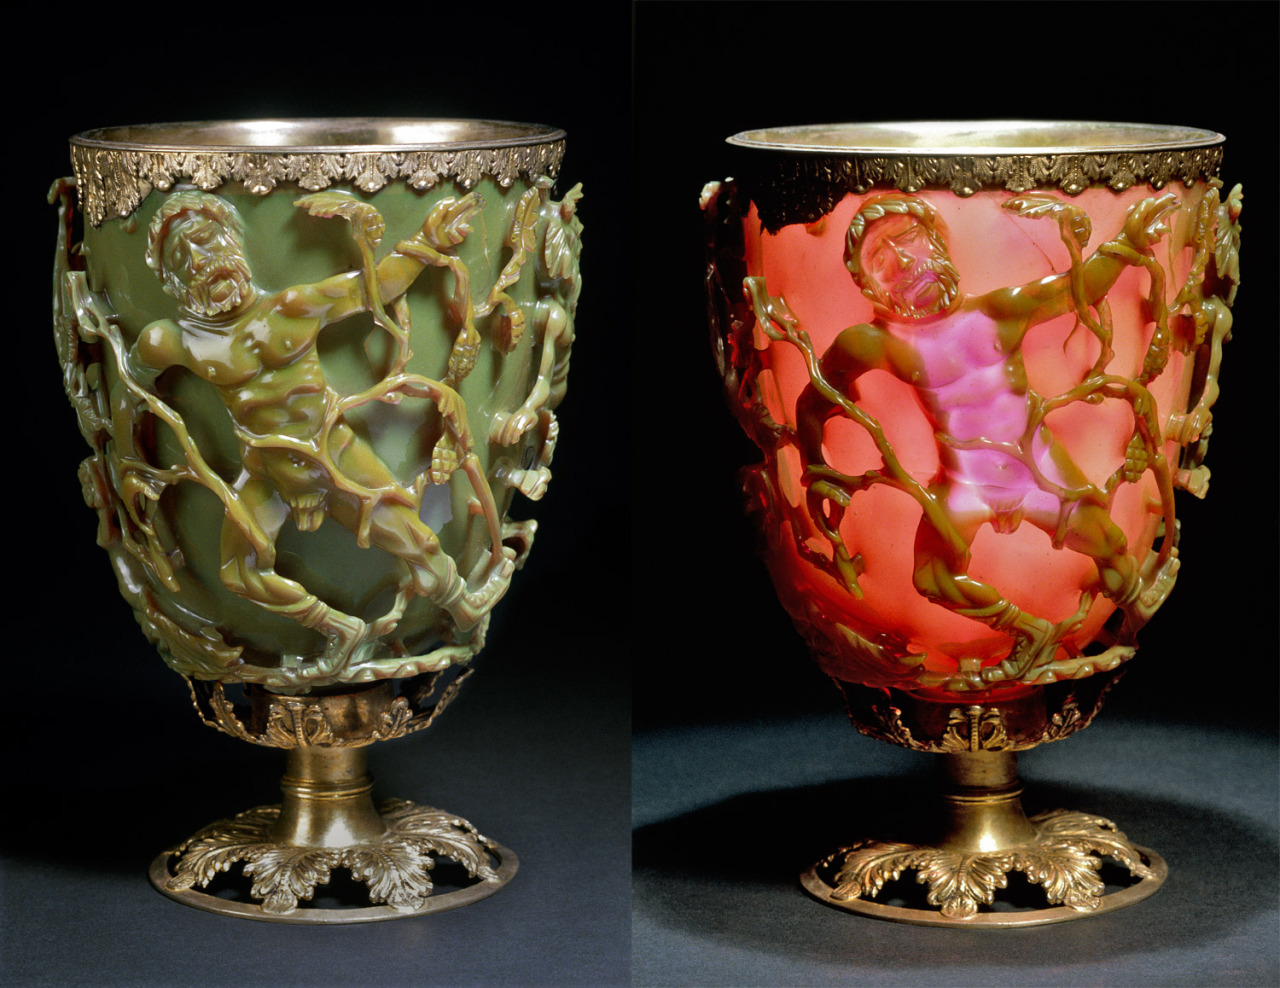
\includegraphics[width = 0.6\textwidth]{Lycurguscup.jpg}
    \caption{La copa de Lycurgo, copa fabricada en la Roma tardía del
      siglo IV D.C., cuya fabricación resultante muestra propiedades
      ópticas excepcionales.  Taza para beber de vidrio verde y rojo
      cubierto con varias escenas que representan la muerte del rey
      Licurgo; borde montado con una banda de adorno de hoja plateada
      dorada, más pie plateado dorado con hojas de parra caladas. ©
      The Trustees of the British Museum.}
    \label{Lycurgus}
\end{figure}
Estudios de la composición del vidrio dan lugar a la conclusión de que
tales propiedades son causadas por la presencia de finas partículas de
oro dispersadas, probablemente una aleación con plata. Con estudios de
microscopía de transmisión de electrones, TEM, por sus siglas en
inglés, se pudieron determinar tamaños de las partículas de $\approx
10 nm $. Actualmente se ha encontrado que contiene partículas de
diferentes metales y de materiales no metálicos.

%¿Agregaríamos algo más, quitamos esto y ponemos los vidrios de la
%catedral?% Falta agregar la última lámina de la presentación de
%ejemplos sobre propiedades ópticas de partículas cúbicas, pero no supe
%como introducirlas.%

\subsection{Electrodinámica}
La descripción de los fenomenos electromagnéticos es provista por las
ecuaciones de Maxwell las cuales describen la propagación de los
campos electromagnéticos en el vacío y en la materia, su interacción
con las cargas eléctricas de los materiales, y la interacción entre las
mismas cargas, las ecuaciones en forma diferencial son,
\begin{equation}
  \label{Maxwell-eqs}
  \begin{array}{cc}
    \nabla \cdot {\bf D} = 4\pi \rho_{ex}, & \nabla \cdot {\bf B} =0, \\
    \nabla \times {\bf E} = -\frac{1}{c}\frac{\partial {\bf B}}{\partial t}, &
    \nabla \times {\bf H} = \frac{4\pi}{c}{\bf
      J}_{ex} + \frac{1}{c}\frac{\partial {\bf D}}{\partial t},
  \end{array}
\end{equation}
donde ${\bf J}_{ex}$ y $\rho_{ex}$ son la densidad de corriente y
densidad de carga externas, respectivamente. Por ejemplo, el siguiente
sistema que consiste de circuitos de alambre a los que se aplica un
campo magnético a lo largo de la dirección perpendicular al plano en
el que está el circuito y un campo eléctrico que reside en el mismo
plano y cuyo efecto sobre los circuitos es el movimiento de sus
caragas eléctricas, como ilustra la figura \ref{circuitos}.
\begin{figure}
  \centering
  

\tikzset{every picture/.style={line width=0.75pt}} %set default line width to 0.75pt        

\begin{tikzpicture}[x=0.75pt,y=0.75pt,yscale=-1,xscale=1]
%uncomment if require: \path (0,300); %set diagram left start at 0, and has height of 300

%Shape: Ellipse [id:dp7618038563365439] 
\draw  [color={rgb, 255:red, 74; green, 100; blue, 226 }  ,draw opacity=1 ][line width=2.25]  (239,162.08) .. controls (239,141.23) and (282.35,124.33) .. (335.83,124.33) .. controls (389.32,124.33) and (432.67,141.23) .. (432.67,162.08) .. controls (432.67,182.93) and (389.32,199.83) .. (335.83,199.83) .. controls (282.35,199.83) and (239,182.93) .. (239,162.08) -- cycle ;
\draw  [color={rgb, 255:red, 74; green, 100; blue, 226 }  ,draw opacity=1 ][fill={rgb, 255:red, 74; green, 97; blue, 226 }  ,fill opacity=1 ] (427.77,163.58) -- (425.05,147.77) -- (440.17,158.66) -- (430.67,156.18) -- cycle ;
%Shape: Ellipse [id:dp40950593076291275] 
\draw  [color={rgb, 255:red, 74; green, 100; blue, 226 }  ,draw opacity=1 ][line width=2.25]  (258.76,161.46) .. controls (258.76,144.73) and (293.31,131.16) .. (335.92,131.16) .. controls (378.52,131.16) and (413.07,144.73) .. (413.07,161.46) .. controls (413.07,178.2) and (378.52,191.77) .. (335.92,191.77) .. controls (293.31,191.77) and (258.76,178.2) .. (258.76,161.46) -- cycle ;
\draw  [color={rgb, 255:red, 74; green, 100; blue, 226 }  ,draw opacity=1 ][fill={rgb, 255:red, 74; green, 97; blue, 226 }  ,fill opacity=1 ] (409.17,162.67) -- (406.99,149.97) -- (419.04,158.72) -- (411.47,156.73) -- cycle ;
%Shape: Ellipse [id:dp350415193172229] 
\draw  [color={rgb, 255:red, 74; green, 100; blue, 226 }  ,draw opacity=1 ][line width=2.25]  (274.44,161.99) .. controls (274.44,148.45) and (302.22,137.47) .. (336.5,137.47) .. controls (370.77,137.47) and (398.56,148.45) .. (398.56,161.99) .. controls (398.56,175.53) and (370.77,186.51) .. (336.5,186.51) .. controls (302.22,186.51) and (274.44,175.53) .. (274.44,161.99) -- cycle ;
\draw  [color={rgb, 255:red, 74; green, 100; blue, 226 }  ,draw opacity=1 ][fill={rgb, 255:red, 74; green, 97; blue, 226 }  ,fill opacity=1 ] (395.42,162.96) -- (393.67,152.69) -- (403.36,159.77) -- (397.28,158.16) -- cycle ;

%Straight Lines [id:da6004675395388991] 
\draw [color={rgb, 255:red, 71; green, 211; blue, 33 }  ,draw opacity=1 ][fill={rgb, 255:red, 68; green, 211; blue, 33 }  ,fill opacity=1 ][line width=1.5]    (341.17,270.33) -- (338.81,35.67) ;
\draw [shift={(338.78,32.67)}, rotate = 449.43] [color={rgb, 255:red, 71; green, 211; blue, 33 }  ,draw opacity=1 ][line width=1.5]    (14.21,-4.28) .. controls (9.04,-1.82) and (4.3,-0.39) .. (0,0) .. controls (4.3,0.39) and (9.04,1.82) .. (14.21,4.28)   ;
%Straight Lines [id:da8123571653101612] 
\draw [color={rgb, 255:red, 208; green, 2; blue, 27 }  ,draw opacity=1 ][line width=1.5]    (164.17,237.83) -- (243.32,198.34) ;
\draw [shift={(246,197)}, rotate = 513.48] [color={rgb, 255:red, 208; green, 2; blue, 27 }  ,draw opacity=1 ][line width=1.5]    (14.21,-4.28) .. controls (9.04,-1.82) and (4.3,-0.39) .. (0,0) .. controls (4.3,0.39) and (9.04,1.82) .. (14.21,4.28)   ;


% Text Node
\draw (310,18.4) node [anchor=north west][inner sep=0.75pt]  [font=\large]  {$\vec{B}$};
% Text Node
\draw (201,180.4) node [anchor=north west][inner sep=0.75pt]  [font=\large]  {$\vec{E}$};
% Text Node
\draw (434.67,165.48) node [anchor=north west][inner sep=0.75pt]  [font=\large]  {$\vec{j}$};


\end{tikzpicture}


  \caption{Circuitos de lazos de metal bajo la aplicación de un campo
    magnético $\vec{B}$ en la dirección perpendicular a al plano del
    circuito y de un campo eléctrico $\vec{E}$ que reside en el plano
    del circuito. El efecto de la aplicación de los campos sobre los
    alambres de metal es el movimiento de cargas eléctricas, la
    densidad de corriente $\vec{j}$. }
\label{Circuitos}

\end{figure}

Los efectos en la materia por perturbaciones externas es descrito por
sus propiedades intrínsecas tales como la permitividad
$\epsilon(\vec{k},\omega)$, la cual describe cuánto es afectado un
material al aplicar un campo eléctrico y la permeabilidad
$\mu(\vec{k},\omega)$, que describe el efecto cuando se aplican campos
magnéticos. A estas cantidades se les denomina funciones respuesta del
sistema y pueden o no depender de $\vec{k}$ el vector de onda la cual
es y $\omega$ la frecuencia de la preturbación, en el espació real
estas dependencias son espacial y temporal respectivamente. Las
diferentes formas de estás funciones dan pie a la clasifición de la
materia, por ejemplo, un medio con permitividad constante $\epsilon$
en todas las direcciones es un medio isotrópico homogéneo, los medios
cuyas funciones respuesta dependen de la dirección y/o del punto en
que se realiza la medición, se les clasifica como anisotrópicos
inhomogenéos.

La propagación de ondas electromagnéticas en los medios es descrita
por estas funciones respuesta, por ejemplo, consideremos un medio
homogéneo con permitividad constante $\epsilon$, la propagación de la
onda está dada por la relación entre el vector de onda y la
frecuencia, la relación de dispersión de la onda al propagarse en el
medio como se ilustra en la imagen \ref{mediohomogneo}, la cual es
amplificada por el factor $\sqrt{\epsilon}$ con respecto a la relación
de dispersión en el vacío.
\begin{figure}
  \centering
  

\tikzset{every picture/.style={line width=0.75pt}} %set default line width to 0.75pt        

\begin{tikzpicture}[x=0.75pt,y=0.75pt,yscale=-1,xscale=1]
%uncomment if require: \path (0,300); %set diagram left start at 0, and has height of 300

%Shape: Rectangle [id:dp2370189011099142] 
\draw   (346.17,40) -- (596.17,40) -- (596.17,224.17) -- (346.17,224.17) -- cycle ;
%Straight Lines [id:da9477212198255883] 
\draw [color={rgb, 255:red, 31; green, 166; blue, 236 }  ,draw opacity=1 ]   (346.17,73.17) -- (471.17,224.17) ;
%Straight Lines [id:da38120967955829277] 
\draw [color={rgb, 255:red, 31; green, 166; blue, 236 }  ,draw opacity=1 ]   (596.17,74.17) -- (471.17,224.17) ;

%Straight Lines [id:da8438048623151154] 
\draw [color={rgb, 255:red, 208; green, 2; blue, 27 }  ,draw opacity=1 ]   (346.17,41.17) -- (471.17,223.17) ;
%Straight Lines [id:da6201464061225517] 
\draw [color={rgb, 255:red, 208; green, 2; blue, 27 }  ,draw opacity=1 ]   (596.17,42.37) -- (471.17,223.17) ;

%Straight Lines [id:da8440907794928258] 
\draw    (471.17,223.17) -- (470.17,40.17) ;

%Shape: Rectangle [id:dp06864759116466967] 
\draw  [color={rgb, 255:red, 31; green, 166; blue, 236 }  ,draw opacity=1 ][fill={rgb, 255:red, 31; green, 166; blue, 236 }  ,fill opacity=1 ] (53.17,41) -- (319.17,41) -- (319.17,225.17) -- (53.17,225.17) -- cycle ;



% Text Node
\draw (299,-107.6) node [anchor=north west][inner sep=0.75pt]  [font=\tiny]  {$\vec{\mathbf{\zeta }}$};
% Text Node
\draw (55.17,228.57) node [anchor=north west][inner sep=0.75pt]    {$( a)$};
% Text Node
\draw (84,68.4) node [anchor=north west][inner sep=0.75pt]  [font=\Large]  {$\epsilon $};
% Text Node
\draw (348.17,227.57) node [anchor=north west][inner sep=0.75pt]    {$( b)$};
% Text Node
\draw (519,157.4) node [anchor=north west][inner sep=0.75pt]  [color={rgb, 255:red, 47; green, 43; blue, 198 }  ,opacity=1 ]  {$k=\sqrt{\epsilon }\frac{\omega }{c}$};
% Text Node
\draw (507,71.4) node [anchor=north west][inner sep=0.75pt]  [color={rgb, 255:red, 208; green, 2; blue, 27 }  ,opacity=1 ]  {$k=\frac{\omega }{c}$};
% Text Node
\draw (465,233.4) node [anchor=north west][inner sep=0.75pt]  [color={rgb, 255:red, 0; green, 0; blue, 0 }  ,opacity=1 ]  {$k$};
% Text Node
\draw (327,121.4) node [anchor=north west][inner sep=0.75pt]    {$\omega $};


\end{tikzpicture}


  \caption{(a) Medio homogéneo con permitividad constante $\epsilon$,
    (b) relaciones de dipersión de la propagación de la onda, línea
    roja propagación en el vacío, línea azul propagación dentro del material.}
\label{mediohomogneo}

\end{figure}


\section{Teoría}

Las propiedades ópticas de estos materiales están determinadas por su
composición y geometría. Propiedades como las relaciones de dispersión
de los modos electromagnéticos que se propagan a través del material
en un sistema semi-infinito, las amplitudes de reflexión y transmisión,
y relaciones de dispersión de modos electromagnéticos en la superficie
de un sistema bordeado pueden ser expresadas en términos del operador
dieléctrico macroscópico a través de las soluciones de las ecuaciones
de Maxwell en dicho material.

Las ecuaciones de Maxwell con las cuales se asume una descripción
macroscópica de los campos en un medio son
\begin{equation}
  \label{Maxwell-eqs}
  \begin{array}{cc}
    \nabla \cdot {\bf D} = 4\pi \rho_{ex}, & \nabla \cdot {\bf B} =0, \\
    \nabla \times {\bf E} = -\frac{1}{c}\frac{\partial {\bf B}}{\partial t}, &
    \nabla \times {\bf H} = \frac{4\pi}{c}{\bf
      J}_{ex} + \frac{1}{c}\frac{\partial {\bf D}}{\partial t},
  \end{array}
\end{equation}
donde ${\bf J}_{ex}$ y $\rho_{ex}$ son la densidad de corriente y
densidad de carga externas, respectivamente. Y para calcular
respuestas ópticas de un sistema se define al operador dieléctrico
$\hat{\epsilon}_{M}$ a través de la relación
\begin{equation}
  {\bf D}_{a} = \hat{\epsilon}_{M} {\bf E}_{a}
  \label{Def-Dilectric-Op}
\end{equation}
donde ${\bf D}_{a}$ y ${\bf E}_{a}$ representan los promedios macroscópicos del
campo desplazamiento y eléctrico, respectivamente.

Sin embargo es posible definir ${\bf D}$ y ${\bf H}$ para incluir
fluctuaciones microscópicas y que sigan obedeciendo las ecuaciones de
Maxwell \eqref{Maxwell-eqs}.

Para poder describir la respuesta óptica de un sistema que incluye
fluctuaciones locales de los campos inducidas por inhomogeneidades del
sistema, consideramos primero una respuesta dieléctrica,
$\hat{\epsilon}$, microscópica
\begin{equation}
  {\bf D} = \hat{\epsilon} {\bf E},
  \label{MicroscopicDielectric-Op}
\end{equation}
la cual acopla las fluctuaciones locales de los campos ${\bf D}$ y
${\bf E}$ totales y a la cual se le aplica un procedimiento de
promediación para relacionar $\hat{\epsilon}$ con
$\hat{\epsilon}_{M}$, de tal manera que las fluctuaciones
microscópicas sean incorporadas en la respuesta macroscópica. Para tal
proposito seguimos el procedimiento descrito en
\cite{ElectromagneticResponseofSystemwithSpatialFluctuations}, por
Mochán et al.

Formalmente se definen los operadores 
\begin{equation}
  \begin{array}{cc}
    \label{operadoresPromedio-Fluctuaciones}
    \hat{P}_{a}, & \hat{P}_{f} = \hat{1} - \hat{P}_{a}, 
  \end{array}
\end{equation}
los cuales extraen la componente promedio $F_{a}=\hat{P}_{a}F$ y
fluctuante $F_{f}=\hat{P}_{f}F$ de una función $F = F_{a}+F_{f}$
arbitraria. Tales operadores son idempotentes
\begin{equation}
  \begin{array}{cc}
    \label{Op-Idempotentes}
    \hat{P}^{2}_{a}=\hat{P}_{a}, & \hat{P}^{2}_{f} =\hat{P}_{f},
  \end{array}
\end{equation}
\begin{equation}
  \hat{P}_{a}\hat{P}_{f}=\hat{P}_{f}\hat{P}_{a}=0,
\end{equation}
lo cual significa que son operadores de proyección.

Consideremos un campo eléctrico consistente de una parte promedio y
una parte fluctuante
\begin{equation}
  {\bf E} = \left(\begin{split} {\bf E}_{a} \\
    {\bf E}_{f} \end{split}\right),
\end{equation}
representado como en la siguiente imagen reescribiendo
\eqref{MicroscopicDielectric-Op} proyectada en los subespacios $a$ y
$f$,
\begin{equation}
  \label{CamposCompletos}
  \left(\begin{split} {\bf D}_{a} \\  {\bf D}_{f} \end{split}\right) =
  \left(\begin{matrix} \hat{\epsilon}_{aa} & \hat{\epsilon}_{af} \\
    \hat{\epsilon}_{fa} & \hat{\epsilon}_{ff} \end{matrix}\right)
  \left(\begin{split} {\bf E}_{a} \\ {\bf E}_{f} \end{split}\right),
\end{equation}
donde se ha definido
\begin{equation}
  \begin{array}{cc}
    \hat{O}_{\alpha \beta}\equiv \hat{P}_{\alpha}\hat{O}\hat{P}_{\beta}, & \alpha,\beta =a,f,
  \end{array}
\end{equation}
para cualquier operador.

Para calcular la respuesta macroscópica del sistema desacoplamos
${\bf D}_{a}$ y ${\bf E}_{f}$ de la ecuación de campos completos
\eqref{CamposCompletos}. Usando las ecuaciones de Maxwell para
los campos microscópicos se encuentra una relación entre ${\bf E}_{a}$
y ${\bf E}_{f}$,
\begin{equation}
  \begin{split}
      \nabla \times \nabla \times {\bf E} = \frac{4\pi
        i\omega}{c^{2}}{\bf j}_{ex} + \frac{\omega^{2}}{c^{2}}{\bf D}
      \\ \left[ \hat{\epsilon}_{ff} - \frac{c^{2}}{\omega^{2}}(\nabla
        \times \nabla \times)_{ff}\right] {\bf E}_{f} = \frac{4\pi}{i
        \omega }{\bf j}_{f}^{ex}-\hat{\epsilon}_{fa}{\bf E}_{a}
  \end{split}
\end{equation}
asumiendo que ${\bf J}^{ex}_{f} = 0 $, sustituimos ${\bf E}_{f}$ en la
ecuación \eqref{CamposCompletos},
\begin{equation}
  {\bf
    D}_{a}=\left(\hat{\epsilon}_{aa}-(\hat{\epsilon}_{af}(\hat{\epsilon}_{ff}-\frac{c^{2}}{\omega^{2}}(\nabla
  \times \nabla)_{ff})^{-1}\hat{\epsilon}_{fa}\right){\bf E}_{a},
  \label{MacroscopicRelation}
\end{equation}
comparando con la ecuación de campos macroscópicos obtenemos que
\begin{equation}
  \hat{\epsilon}_{M}=\hat{\epsilon}_{aa}-\hat{\epsilon}_{af}\left[(\hat{\epsilon}_{ff}-\frac{c^{2}}{\omega^{2}}(\nabla
    \times \nabla)_{ff})\right]^{-1}\hat{\epsilon}_{fa},
  \label{DielectricFunction}
\end{equation}
la respuesta macroscópica de un sistema está dada por el promedio de
su respuesta microscópica, más una corrección debida al acoplamiento
entre las componentes fluctuante y promedio de los campos, éste
resultado se presume exacto.

Para analizar el resultado de \eqref{DielectricFunction} nos
restringimos a una longitud de escala característica de las
fluctuaciones mucho menor a la longitud de onda. Convenitntemente se
definen los operadores de proyección longitudinal
\begin{equation}
  \hat{P}^{L} = \hat{\nabla} \hat{\nabla}^{-2} \hat{\nabla}\times,
\end{equation}
y transversal
\begin{equation}
  \hat{P}^{T}=-\hat{\nabla}\times \hat{\nabla}^{-2} \hat{\nabla}\times,
\end{equation}
tales que extraen las partes irrotacional ${\bf F}^{L}=\hat{P}^{L}{\bf
  F} $ y solenoidal ${\bf F}^{T}=\hat{P}^{T}{\bf F}$ de una campo
vectorial arbitrario. Estos operadores cumplen las siguiente
propiedades
\begin{equation}
  \begin{array}{cc}
    \hat{P}^{T}\hat{P}^{T}=\hat{P}^{T}, & \hat{P}^{L}\hat{P}^{L}=\hat{P}^{L},\\
    \hat{P}^{T}\hat{P}^{L}=\hat{P}^{L}\hat{P}^{T}=0, & \hat{P}^{T}+\hat{P}^{L}=\hat{1},
  \end{array}
\end{equation}
y communtan con $\hat{P}_{f}$ y $\hat{P}_{a}$.

Al proyectar $\hat{\mathcal{W}}^{-1}=
\left[(\hat{\epsilon}_{ff}-\frac{c^{2}}{\omega^{2}}(\nabla \times
  \nabla \times)_{ff})\right]^{-1}$ en los subespacios longitudina y
transversal
\[\hat{\mathcal{W}}^{-1}=\left[
    \begin{array}{cc}
    \mathcal{W}_{LL} &  \mathcal{W}_{LT} \\
    \mathcal{W}_{TL} &  \mathcal{W}_{TT}
    \end{array}
    \right]^{-1}, \] y reescribiendo el termino de operadores nabla
como, $(\nabla \times \nabla \times)_{ff} = \nabla
^{2}\hat{P}^{T}\hat{P}_{f}$, tenemos
\begin{equation}
  \label{MatrizdeProyeccionesdeW}
  \left[(\hat{\epsilon}_{ff}-\frac{c^{2}}{\omega^{2}}(\nabla \times \nabla \times)_{ff})\right]^{-1} = \left[
  \begin{array}{cc}
    \hat{\epsilon}_{ff}^{LL} & \hat{\epsilon}_{ff}^{LT}
    \\ \hat{\epsilon}_{ff}^{TL} & \hat{\epsilon}_{ff}^{TT}+
    \frac{c^{2}}{\omega^{2}}\nabla ^{2}\hat{P}^{T}\hat{P}_{f}
  \end{array}
  \right]^{-1}.
\end{equation}

La manera en que obtenemos las componentes de la matriz es la
siguiente, definimos una matriz y su inversa

\[ \hat{M} = \left(
\begin{array}{cc}
  \hat{A} &  \hat{B} \\
   \hat{C} &  \hat{D}
\end{array}\right),
\] 
\[ \hat{m} =\left( 
\begin{array}{cc}
   \hat{a} &  \hat{b} \\
   \hat{c} &  \hat{d}
\end{array}\right) = \hat{M}^{-1},
\] 
la cuales deben cumplir con las ecuaciones
\begin{equation}
  \begin{split}
    \hat{A} \hat{a}+ \hat{B} \hat{c} = 1, \\
    \hat{A} \hat{b}+ \hat{B} \hat{d} = 0, \\
    \hat{C} \hat{a}+ \hat{D} \hat{c} = 0, \\
    \hat{C} \hat{b}+ \hat{D} \hat{d} = 1,
  \end{split}
\end{equation}
de las cuales uno despeja
\begin{equation}
  \label{eqsalgebraicas}
  \begin{split}
    \hat{a} = \hat{A}^{-1}(1-\hat{B}\hat{D}^{-1}\hat{C}\hat{A}^{-1})^{-1}, \\
    \hat{b} = \hat{C}^{-1}(1-\hat{D}\hat{B}^{-1}\hat{A}\hat{C}^{-1})^{-1}, \\
    \hat{c} = - \hat{D}^{-1}\hat{C}\hat{A}^{-1}(1-\hat{B}\hat{D}^{-1}\hat{C}\hat{A}^{-1})^{-1}, \\
    \hat{d} = - \hat{B}^{-1}\hat{A} \hat{C}^{-1}(1-\hat{D}\hat{B}^{-1}\hat{A}\hat{C}^{-1})^{-1}.
  \end{split}
\end{equation}

Para usar este desarrollo definimos $\hat{M} = \hat{\mathcal{W}}$ por
lo que los elementos respectivos son
\[
\begin{split}
  \hat{A} = \hat{\epsilon}_{ff}^{LL}, \\
  \hat{B} = \hat{\epsilon}_{ff}^{LT}, \\
  \hat{C} = \hat{\epsilon}_{ff}^{TL}, \\
  \hat{D} = \hat{\epsilon}_{ff}^{TT}+\frac{c^{2}}{\omega^{2}}\nabla ^{2}\hat{P}^{T}\hat{P}_{f},
\end{split}
\]
y asumiendo que $\lambda^{2}/l^{2} >> ||\hat{\epsilon}||$ donde $l$ es
la longitud de escala de las fluctuaciones, y que
$||(\omega^{2}/c^{2})\hat{\nabla}^{-2}\hat{P}_{f}||\approx
l^{2}/\lambda ^{2}$, entonces el segundo termino del elemento
$\hat{D}$ es mucho mayor que el primero. Para hacer el cálculo más
explícito lo reescribimos como
\[ \frac{c^{2}}{\omega^{2}}\nabla ^{2}\hat{P}^{T}\hat{P}_{f}(1+\frac{\omega^{2}}{c^{2}}\nabla ^{-2}\hat{P}^{T}\hat{P}_{f}\hat{\epsilon}_{ff}^{TT}) \]
y al sustituir en las ecuaciones \eqref{eqsalgebraicas}, obtenemos
\begin{equation}
  \begin{split}
    &\left[(\hat{\epsilon}_{ff}- \frac{c^{2}}{\omega^{2}}(\nabla \times
      \nabla \times)_{ff})\right]^{-1}  =
    \left[ \begin{array}{cc}
        (\hat{\epsilon}_{ff}^{LL})^{-1} & 0 \\ 0 & 0 \\
    \end{array}
      \right] \\ & + \frac{\omega^{2}}{c^{2}}\left[ \begin{array}{cc}
        (\hat{\epsilon}_{ff}^{LL})^{-1}(\hat{\epsilon}_{ff}^{LT})\hat{\nabla}^{-2}(\hat{\epsilon}_{ff}^{TL})(\hat{\epsilon}_{ff}^{LL})^{-1}
        &
        -(\hat{\epsilon}_{ff}^{LL})^{-1}(\hat{\epsilon}_{ff}^{LT})\hat{\nabla}^{-2}
        \\ -\hat{\nabla}^{-2}(\hat{\epsilon}_{ff}^{TL})(\hat{\epsilon}_{ff}^{LL})^{-1}
        & \nabla^{-2}\hat{P}^{T}\hat{P}_{f}
      \end{array} \right] + ...,
    \end{split}
\end{equation}
en los casos en que $l << \lambda $, solo nos quedamos con el primer
termino de la expansión y sustituyéndolo en \eqref{DielectricFunction}
la reescribimos como
\begin{equation}
  \hat{\epsilon}_{M}=\hat{\epsilon}_{aa}-\hat{\epsilon}_{af}(\hat{\epsilon}_{ff}^{LL})^{-1}\hat{\epsilon}_{fa}.
\end{equation}



\section{Implementación}
\section{Resultados}

\begin{thebibliography}{0000}
\bibitem{Metamorphose} Virtual Institute for Artificial
  Electromagnetic Materials and
  Meta-materials. \url{https://www.metamorphose-vi.org/}
\bibitem{IntroductiontoMetamaterialsandNanophotonics} An introduction
  to metamaterials and nanophotonics / Constantin Simovski and Sergei
  Tretyakov, Department of Electronics and Nanoengineering, School of
  Electrical Engineering, Aalto University,
  Finland. \url{http://www.cambridge.org/9781108492645}
\bibitem{ElectromagneticResponseofSystemwithSpatialFluctuations}
  Electromagnetic response of systems with spatial
  fluctuations. I. General formalism. W. Luis Mochán and Rubén
  G. Barrera. Phys. Rev. B 32, 4984 – Published 15 October 1985
\bibitem{Bulkplasmon} Mochán W.L., Plasmons. In: Saleem Hashmi
  (editor-in-chief), Reference Module in Materials Science and
  Materials. Engineering. Oxford: Elsevier; 2016. pp. 1-13. ISBN:
  978-0-12-803581-8. Copyright © 2016 Elsevier Inc. unless otherwise
  stated. All rights reserved.
\bibitem{LycurgusInvestigation} Barber DJ, Freestone IC (1990) An
  investigation of the origin of the color of the Lycurgus cup by
  analytical transmission electron-microscopy. Archaeometry 32:33–45

  
  \end{thebibliography}

\end{document}
